\documentclass[10pt, twocolumn]{article}

\usepackage[margin=0.75in]{geometry}
\usepackage{amsmath,amsthm,amssymb,bm}
\usepackage{xcolor}
\usepackage{cancel}
\usepackage{graphicx}
\usepackage{changepage}
\usepackage{circuitikz}
\usepackage{pgfplots}
\usepackage{minted}
\usepackage{physics}
\usepackage{tikz}
\usepackage{tikz-3dplot}
\usepackage{hyperref}
\usepackage{cleveref}
\usepackage[uncertainty-mode = separate, separate-uncertainty-units = single]{siunitx}
\usepackage{fontspec}
\usepackage{relsize}
\usepackage{subcaption}
\usepackage{todonotes}
\usepackage{multicol, multirow, booktabs}
\usepackage[breakable]{tcolorbox}
\usepackage[inline]{enumitem}

\theoremstyle{definition}
\newtheorem{problem}{Problem}
\newtheorem{soln}{Solution}

\pgfplotsset{compat=newest}
\usetikzlibrary{lindenmayersystems}
\usetikzlibrary{arrows}
\usetikzlibrary{calc}
\usetikzlibrary{positioning, fit}
\usetikzlibrary{3d, perspective}
\usetikzlibrary{math}
\usetikzlibrary{fadings}
\usetikzlibrary{angles,quotes} 

\definecolor{incolor}{HTML}{303F9F}
\definecolor{outcolor}{HTML}{D84315}
\definecolor{cellborder}{HTML}{CFCFCF}
\definecolor{cellbackground}{HTML}{F7F7F7}
\newcommand{\bv}[1]{\bm{\mathrm{#1}}}
\newcommand{\ui}{\bv{\hat{i}}}
\newcommand{\uj}{\bv{\hat{j}}}
\newcommand{\uk}{\bv{\hat{k}}}
\newcommand{\ux}{\bv{\hat{x}}}
\newcommand{\uy}{\bv{\hat{y}}}
\newcommand{\uz}{\bv{\hat{z}}}
\newcommand{\uv}[1]{\hat{\bv{{#1}}}}
\newcommand{\pd}[2][]{{\frac{\partial^{#1}}{\partial {{#2}^{#1}}}}}
\newcommand{\dif}[2][]{{\frac{d^{#1}}{d{{#2}^{#1}}}}}
\newcommand{\grd}{\nabla}

\pgfdeclarelayer{background}  
\pgfsetlayers{background,main}
\AtBeginDocument{\RenewCommandCopy\qty\SI}

\makeatletter
\newcommand{\boxspacing}{\kern\kvtcb@left@rule\kern\kvtcb@boxsep}
\makeatother
\newcommand{\prompt}[4]{
    \ttfamily\llap{{\color{#2}[#3]:\hspace{3pt}#4}}\vspace{-\baselineskip}
}

\newcommand{\thevenin}[2]{
  \begin{center}
    \begin{circuitikz} \draw
      (0,0) -- (2,0) to[battery1, l_=$V_{Th}\eq#1$] (2,2) 
      to[resistor, l_=$R_{Th}\eq#2$] (0,2)
      ;
      \draw [o-] (-.07,2.079);
      \draw [o-] (-.07,0.079);
    \end{circuitikz}
  \end{center}
}

\newcommand{\norton}[2]{
  \begin{center}
    \begin{circuitikz} \draw
      (0,0) -- (3,0) to[american current source, l_=$I_{N}\eq#1$] (3,2) -- (0,2) (2,0)
      to[resistor, l=$R_{N}\eq#2$] (2,2)
      ;
      \draw [o-] (-.07,2.079);
      \draw [o-] (-.07,0.079);
    \end{circuitikz}
  \end{center}
}

\DeclareMathOperator{\Div}{div}
\DeclareMathOperator{\Curl}{curl}
\DeclareMathOperator{\sgn}{sgn}

\newcommand{\highlight}[1]{\colorbox{yellow}{$\displaystyle #1$}}

\newcommand{\ti}[1]{\widetilde{#1}}

\newfontface{\Kaufmann}{Kaufmann}
\DeclareTextFontCommand{\kf}{\Kaufmann}
\newcommand{\scriptr}{\fontsize{12pt}{12pt}\kf{r}\fontsize{10pt}{10pt}}

\newfontface{\KaufmannB}{Kaufmann Bold}
\DeclareTextFontCommand{\kfb}{\KaufmannB}
\newcommand{\bscriptr}{\fontsize{12pt}{12pt}\kfb{r}\fontsize{10pt}{10pt}}
\newcommand{\justif}[2]{&{#1}&\text{#2}}

\title{Physics 3200Y: Lab 4}
\author{Jeremy Favro (0805980), Bryan Roberts (0691165), Melodie Johnston (0794390)
 \\\emph{Department of Physics \& Astronomy}\\ Trent University, Peterborough, ON, Canada}
\date{\today}


\begin{document}

\maketitle
\begin{abstract}

\end{abstract}
\section{Introduction}
This lab seeks to develop and test theoretical models for the field between two current carrying loops of wire. The developed models predict a high uniformity of the magnetic field between the coils in both magnitude and direction. The theoretical uniformity of the field will be investigated through the construction of the structure for which models were derived and the use of a magnetic field probe.
Additionally the more mathematically challenging off-axis field of the coil structure will be measured and investigated.

\section{Theory}
\begin{figure}[H]
  \centering
  \begin{subfigure}[t]{0.5\textwidth}
    \centering
    \tdplotsetmaincoords{74}{120}
    \begin{tikzpicture}[scale=2, tdplot_main_coords]
      % Axis
      \draw[->] (3,0,0) -- (-3,0,0) node[above right]{$y$};
      \draw[->] (0,-2,0) -- (0,2,0) node[right]{$x$};
      \draw[->] (0,0,-1.5) -- (0,0,1.5) node[above]{$z$};

      % Circular Loops
      \draw[line width = 1.2mm, orange] (0,0,1) circle [radius=1];
      \draw[line width = 1.2mm, orange] (0,0,-1) circle [radius=1];

      \draw (0,0,-1) -- (0,0,0.5);
      \draw[->] (0,0,0.9) -- (0,0,1.5);

      % Radius
      \draw [->] (0,0,1) -- (1,0,1) node [midway, above] {\small$R$} ;
      \draw [->] (0,0,-1) -- (1,0,-1) node [midway, above] {\small$R$} ;

      % Center Distance
      \draw[|<-] (2.2,0,1.54) -- (2.2,0,0.7) node [below] {\small$R$};
      \draw[->|] (2.2,0,0.41)-- (2.2,0,-0.46) ;

      % Current Direction
      \draw [line width = 0.7mm, blue, ->] (1.4,-0.1,1) arc (-20:20:1.1) node [black, midway, below] {$I$};
      \draw [line width = 0.7mm, blue, ->] (1.4,-0.1,-1) arc (-20:20:1.1) node [black, midway, below] {$I$};
    \end{tikzpicture}
  \end{subfigure}%
  % ~
  % \begin{subfigure}[t]{0.5\textwidth}
  %   \centering
  %   \tdplotsetmaincoords{90}{120}
  %   \begin{tikzpicture}[scale=2, tdplot_main_coords]
  %     % Axis
  %     \draw[->] (0,-2,0) -- (0,2,0) node[right]{$x$};
  %     \draw[->] (0,0,-1.5) -- (0,0,1.5) node[above]{$z$};

  %     % Circular Loops
  %     \draw[line width = 1.2mm, orange] (0,0,1) circle [radius=1];
  %     \draw[line width = 1.2mm, orange] (0,0,-1) circle [radius=1];

  %     % Refinements for 3d View
  %     \draw (0,0,-1) -- (0,0,0.5);
  %     \draw[->] (0,0,0.9) -- (0,0,1.5);

  %     % Radius
  %     \draw [->] (0,0,1) -- (0,1.1,1) node [midway, above] {$R$} ;

  %     % Center Distance
  %     \draw[|<->|] (2.2,0,-1) -- (2.2,0,1) node [midway, above right] {$R$};

  %     % Current Direction
  %     \draw [line width = 0.7mm, blue, ->] (1.4,-0.1,1) arc (-20:20:1.1) node [black, midway, below] {$I$};
  %     \draw [line width = 0.7mm, blue, ->] (1.4,-0.1,-1) arc (-20:20:1.1) node [black, midway, below] {$I$};
  %   \end{tikzpicture}
  %   \caption{Side-on view of the coils}
  % \end{subfigure}
  \caption{Helmholtz coil structure}
  \label{diagram:coils}
\end{figure}
The construction under study, known as Helmholtz coils \todo{Cite?} is illustrated in \cref{diagram:coils}. We consider two coils, each of radius $R$, separated by a distance $R$. In the figure, and for the following derivation, the coils are placed at $\pm R/2$ respectively with the origin between them as indicated in the figure. We begin by deriving the field due to a single current carrying loop and then utilize linear superposition to determine the total magnetic field due to a true Helmholtz coil system. The magnetic field for a wire loop represented by a (directed) contour $\mathcal{C}$ is given by the Biot-Savart law,
\begin{equation}
  \bv{B}(\bv{r})=\frac{\mu_0 I}{4\pi}\int_\mathcal{C}\frac{d\bv{\ell}'\times \bscriptr'}{\scriptr^3}
  \label{eq:biot-savart}
\end{equation}
where $\bscriptr=\bv{r}-\bv{r}'$ and $\bv{r}$ and $\bv{r}'$ represent the test-point and an integration variable respectively.
To exploit the symmetries present in the problem we consider only the field on the axis of symmetry, hereon referred to as the on-axis field. This means that our position vector $\bv{r}=(0,0,z)$ in cylindrical coordinates. Since we are considering only the field due to a single coil we take $\bv{r}'=R\uv{s}$ which sweeps out the entire coil. This gives $\bscriptr=z\uz-R\uv{s}$. Finally if we direct the contour such that the area vector is in $\uz$, $d\ell'=Rd\phi'\uv{\phi}$. This means that \cref{eq:biot-savart} becomes
\begin{align*}
  \bv{B}(\bv{r}) & =\frac{\mu_0 I}{4\pi}\int_0^{2\pi}\frac{Rd\phi'z\uv{s}+R^2d\phi'\uz}{(z^2+R^2)^{3/2}} \\
                 & =\frac{\mu_0 I}{2}\frac{R'z\uv{s}+R^2\uz}{(z^2+R^2)^{3/2}}
\end{align*}
and since the magnetic field obeys linear superposition, $N$ such coils very close together create a field given by
\begin{equation}
  \bv{B}(\bv{r})=\frac{\mu_0 NI}{2}\frac{R'z\uv{s}+R^2\uz}{(z^2+R^2)^{3/2}}.
  \label{eq:nfield}
\end{equation}
Now we can construct the field due to two such coils at $\pm R/2$ easily again by linear superposition,
\begin{align}
  \bv{B}(\bv{r}) & =\frac{\mu_0 NIR^2}{2}\left[\frac{1}{((z+R/2)^2+R^2)^{3/2}}\right.\nonumber \\
                 & \quad+\left.\frac{1}{((z-R/2)^2+R^2)^{3/2}}\right]\uz
  \label{eq:helmholtz-field}
\end{align}
where we've canceled out the $\uv{s}$ components of the field by symmetry.
We can plot this expression (in natural units),
\begin{figure}[h]
  \centering
  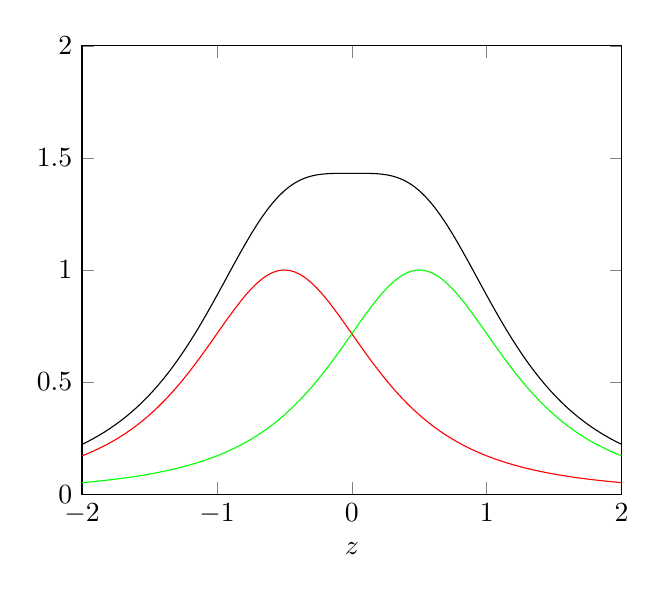
\begin{tikzpicture}
    \begin{axis}[
        domain=-2:2,
        xmin=-2, xmax=2,
        ymin=0, ymax=2,
        samples=100,
        xlabel=$z$
      ]
      \addplot[mark=none, red] {1/((x+1/2)^2+1)^(1.5)};
      \addplot[mark=none, green] {1/((x-1/2)^2+1)^(1.5)};
      \addplot[mark=none] {(1/((x-1/2)^2+1)^(1.5))+(1/((x+1/2)^2+1)^(1.5))};
    \end{axis}
  \end{tikzpicture}
  \caption{Helmholtz coil relative magnetic field strength. The coloured curves are fields due to the individual coils, placed at $\pm 1/2$, and the black curve is their sum.}
\end{figure}
and we see that indeed the field inside and near the center is highly uniform. This is the desired effect of the Helmholtz configuration.
\section{Methods}
\subsection{Coils}
Two 200 turn, $\qty{10}{\centi\meter}$ radius, Pasco Scientific Helmholtz coils were used \cite{pascoHelmholtzCoils}. These were mounted on a ruled base, also manufactured by Pasco Scientific.
\subsection{Magnetic Probe}
The magnetic field produced by the coils was measured using a Pasco Scientific 2-axis field sensor \cite{pascoPASPORT2Axis}. The probe was positioned to measure the fields both perpendicular and parallel to the coil plane to verify the uniformity and self-canceling behaviour in these directions.
Data was collected on the field in several configurations in order to verify the validity of assumptions made in theoretical derivations. Further discussion is available in the results section.
\subsection{Linear Motion Sensor}
In order to measure the field as a function of position in the coil a Pasco Scientific rotary motion sensor \cite{pascoPASPORTRotary} was used, with the magnetic field probe mounted to a rigid support whose extension into the coils could be tracked by the motion sensor.
\subsection{Alignment}
A challenge in configuring the experiment was the need to measure as closely as possible to
the axis of symmetry of the coils, as this is the region in which the theory derived previously applies. To align the probe vertically two rulers were placed perpendicularly and the axial field indicator dot on the probe was aligned with the appropriate position on the rulers. To align horizontally a similar process was used except with the perpendicular field indicator dot. The motion sensor was zeroed at $\qty{10}{\centi\meter}$ from the first coil. \todo{Make some pictures of the setup here and shunt results to next page}
\section{Results}
\subsection{On-Axis}
The on-axis field was collected in several configurations. These are: the normal Helmholtz configuration, one coil on and the other off for each coil, both coils at a separation of $2R$, and
both coils at a separation of $R/2$. For each run the current passing through the coils was held at a value not exceeding $\qty{1.5}{\ampere}$, though due to coil heating a drop to as low as $\qty{1.47}{\ampere}$ was observed.
% STANDARD HOLTZ CONFIG
\begin{figure}[h]
  \centering
  \begin{tikzpicture}
    \begin{axis}[
        xlabel={Position $(\unit{\meter})$},
        ylabel={Field Strength (Gauss)},
        legend style={at={(0.4,0.5)},anchor=south west}
      ]
      \addplot[only marks, color=blue!80!black] table [x=pos, y=axial, col sep=comma] {run1-out.csv};
      \addlegendentry{Axial Field}
      \addplot[mark=none, domain=-0.08:0.08] {((1.256*10^(-6))*1.47*200*(0.1)^2/2)*((1/((x-0.1/2)^2+0.1^2)^(1.5))+(1/((x+0.1/2)^2+0.1^2)^(1.5)))*10000};
      \addlegendentry{Theory}
      \addplot[only marks, color=green!80!black] table [x=pos, y=perp, col sep=comma] {run1-out.csv};
      \addlegendentry{Perpendicular Field}
    \end{axis}
  \end{tikzpicture}
  \caption{Perpendicular and axial fields in a standard Helmholtz configuration.}
  \label{fig:helmholtz-field-data}
\end{figure}
% 2R CONFIG
\begin{figure}[h]
  \centering
  \begin{tikzpicture}
    \begin{axis}[
        xlabel={Position $(\unit{\meter})$},
        ylabel={Field Strength (Gauss)},
        legend style={at={(0.3,0.28)},anchor=south west}
      ]
      \addplot[only marks, color=blue!80!black] table [x=pos, y=axial, col sep=comma] {run4-out.csv};
      \addlegendentry{Axial Field}
      \addplot[mark=none, domain=-0.1:0.1] {((1.256*10^(-6))*1.5*200*(0.1)^2/2)*((1/((x-0.1)^2+0.1^2)^(1.5))+(1/((x+0.1)^2+0.1^2)^(1.5)))*10000};
      \addlegendentry{Theory}
      \addplot[only marks, color=green!80!black] table [x=pos, y=perp, col sep=comma] {run4-out.csv};
      \addlegendentry{Perpendicular Field}
    \end{axis}
  \end{tikzpicture}
  \caption{Perpendicular and axial fields in a $2R$ Helmholtz configuration.}
  \label{fig:helmholtz-2r-field-data}
\end{figure}
% R/2 CONFIG
\begin{figure}[h]
  \centering
  \begin{tikzpicture}
    \begin{axis}[
        xlabel={Position $(\unit{\meter})$},
        ylabel={Field Strength (Gauss)},
        legend style={at={(0.3,0.35)},anchor=south west}
      ]
      \addplot[only marks, color=blue!80!black] table [x=pos, y=axial, col sep=comma] {run5-out.csv};
      \addlegendentry{Axial Field}
      \addplot[mark=none, domain=-0.08:0.08] {((1.256*10^(-6))*1.5*200*(0.1)^2/2)*((1/((x-0.1/4)^2+0.1^2)^(1.5))+(1/((x+0.1/4)^2+0.1^2)^(1.5)))*10000};
      \addlegendentry{Theory}
      \addplot[only marks, color=green!80!black] table [x=pos, y=perp, col sep=comma] {run5-out.csv};
      \addlegendentry{Perpendicular Field}
    \end{axis}
  \end{tikzpicture}
  \caption{Perpendicular and axial fields in an $R/2$ Helmholtz configuration.}
  \label{fig:helmholtz-r/2-field-data}
\end{figure}
\subsubsection{Superposition}
\todo{Figure out a good way to do this}
\subsection{Off-Axis}
Blah blah
\begin{figure}[h]
  \centering
  \begin{tikzpicture}
    \begin{axis}[
      xlabel={$\perp$ Position $(\unit{\meter})$},
      ylabel={$\parallel$ Position $(\unit{\meter})$},
      zlabel={Field Strength (Gauss)}
      legend style={at={(0.3,0.35)},anchor=south west}
      ]
      \addplot3[only marks, color=blue!80!black] table [x=pos, y=fakepos, z=axial, col sep=comma] {run6-out.csv};
      \addlegendentry{$\qty{1.5}{\centi\meter}$}
      \addplot3[only marks, color=green!80!black] table [x=pos, y=fakepos, z=axial, col sep=comma] {run7-out.csv};
      \addlegendentry{$\qty{3}{\centi\meter}$}
      \addplot3[only marks, color=red!80!black] table [x=pos, y=fakepos, z=axial, col sep=comma] {run8-out.csv};
      \addlegendentry{$\qty{5}{\centi\meter}$}
      \addplot3[only marks, color=black] table [x=pos, y=fakepos, z=axial, col sep=comma] {run9-out.csv};
      \addlegendentry{$\qty{8}{\centi\meter}$}
    \end{axis}
  \end{tikzpicture}
  \caption{Perpendicular and axial fields in an $R/2$ Helmholtz configuration.}
  \label{fig:helmholtz-3d-field-data}
\end{figure}
\begin{figure}[h]
  \centering
  \begin{tikzpicture}
    \begin{axis}[
      xlabel={$\perp$ Position $(\unit{\meter})$},
      ylabel={$\parallel$ Position $(\unit{\meter})$},
      zlabel={Field Strength (Gauss)}
      legend style={at={(0.3,0.35)},anchor=south west}
      ]
      \addplot3[only marks, color=blue!80!black] table [x=pos, y=fakepos, z=perp, col sep=comma] {run6-out.csv};
      \addplot3[only marks, color=blue!80!black] table [x=pos, y=fakepos, z=perp, col sep=comma] {run7-out.csv};
      \addplot3[only marks, color=blue!80!black] table [x=pos, y=fakepos, z=perp, col sep=comma] {run8-out.csv};
      \addplot3[only marks, color=blue!80!black] table [x=pos, y=fakepos, z=perp, col sep=comma] {run9-out.csv};
      % \addlegendentry{Axial Field}
      % \addplot[only marks, color=green!80!black] table [x=pos, y=perp, col sep=comma] {run5-out.csv};
      % \addlegendentry{Perpendicular Field}
    \end{axis}
  \end{tikzpicture}
  \caption{Perpendicular and axial fields in an $R/2$ Helmholtz configuration.}
  \label{fig:helmholtz-3d-field-data}
\end{figure}
\section{Discussion}

\bibliographystyle{plain}
\bibliography{sources}
\end{document}
